%% The first command in your LaTeX source must be the \documentclass command.
\documentclass[acmtog,nonacm]{acmart}

%%
%% Define custom colors.
\definecolor{requestedColor}{rgb}{0.97,0,0.30}
\definecolor{personalColor}{rgb}{0,0.7,0.2}

%%
%% \BibTeX command to typeset BibTeX logo in the docs
\AtBeginDocument{%
  \providecommand\BibTeX{{%
    \normalfont B\kern-0.5em{\scshape i\kern-0.25em b}\kern-0.8em\TeX}}}

%%
%% The majority of ACM publications use numbered citations and
%% references.  The command \citestyle{authoryear} switches to the
%% "author year" style.
\citestyle{acmauthoryear}

%%
%% end of the preamble, start of the body of the document source.
\begin{document}

%%
%% The "title" command has an optional parameter,
%% allowing the author to define a "short title" to be used in page headers.
\title{CSE 490V Final Project Report}
\subtitle{Extended Subtitle}

%%
%% The "author" command and its associated commands are used to define
%% the authors and their affiliations.
%% Of note is the shared affiliation of the first two authors, and the
%% "authornote" and "authornotemark" commands
%% used to denote shared contribution to the research.
\author{Student One}
\email{student1@cs.washington.edu}
\author{Student Two}
\email{student2@cs.washington.edu}
\affiliation{\institution{University of Washington}}

%%
%% The abstract provides an overview of the project, including the goals, contributions relative to related work, and the results achieved and documented in this report.
\begin{abstract}
This is the project abstract. This should be a one-paragraph summary, including the motivations, contributions relative to related work, the results achieved and documented in this report, and promising directions for future work. From the project title, the teaser image, and this abstract, most readers should be able to understand most of what your project is about.
\end{abstract}

%%
%% By default, the full list of authors will be used in the page
%% headers. Often, this list is too long, and will overlap
%% other information printed in the page headers. This command allows
%% the author to define a more concise list
%% of authors' names for this purpose.
%\renewcommand{\shortauthors}{Trovato and Tobin, et al.}

%% A "teaser" image appears between the author and affiliation
%% information and the body of the document, and typically spans the
%% page.
\begin{teaserfigure}
  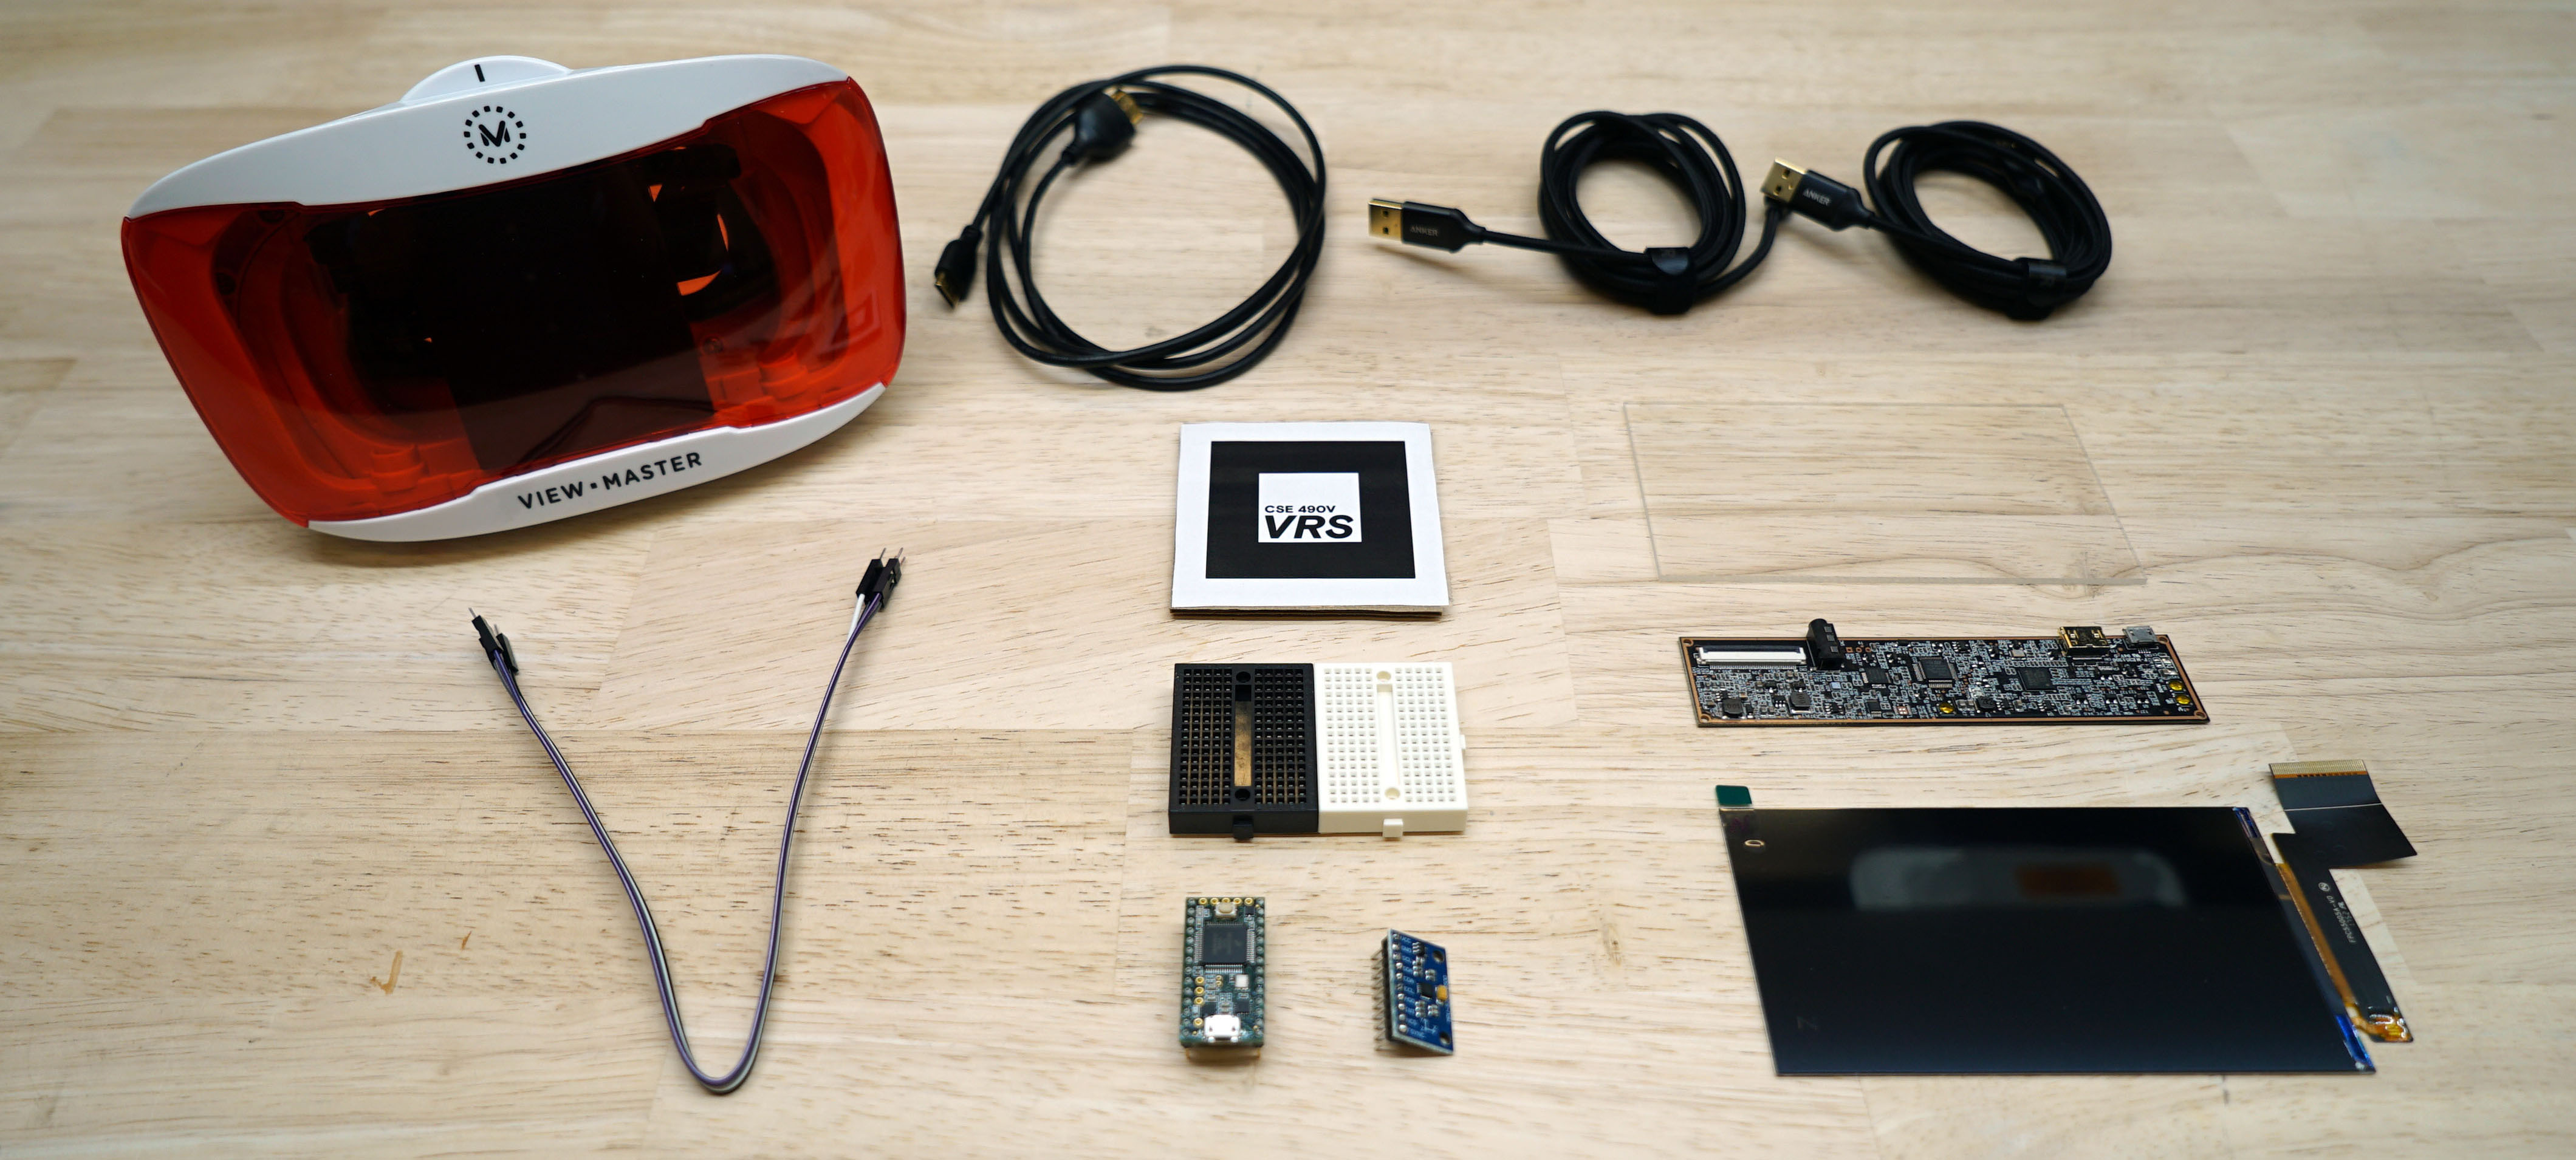
\includegraphics[width=\textwidth]{figures/teaser.jpg}
  \caption{This is the teaser figure. You should select a representative image for your project, such as a photo of any device you built or a screenshot of the application you developed. Write a caption that explains the image(s) in your teaser. For this example the following caption would be suitable. In CSE 490V, students were provided this kit to build their own head-mounted display, including an LCD, an HDMI driver board, an inertial measurement unit (IMU), lenses, an enclosure, and all cabling. All software was developed through the homework assignments.}
  \vspace{1em}
  \label{fig:teaser}
\end{teaserfigure}

%%
%% This command processes the author and affiliation and title
%% information and builds the first part of the formatted document.
\maketitle

\section{Introduction}

\textbf{Remember to update the title, subtitle (if needed), author information, and other details. Please don't submit a report with ``CSE 490V Final Project Report'' as the title!} The introduction is essentially an extended abstract. It is typically 3 to 5 paragraphs long and provides a strong motivation (i.e., why you think this is a useful project to undertake). It should also outline the most important related work (i.e., other publications, products, or similar items that you're improving upon or offering alternatives to). The introduction should also outline what novel approach you're taking or a specific hypothesis you have. You should summarize what you found in this project, as well as what it might mean for future work in this topic.

\subsection{Contributions}

To conclude the introduction, you should provide a concise list of contributions you have made through this project. These should be complete sentences, as shown in the project report examples. Each item should tie to something specific you achieved (e.g., an  idea you introduced, an algorithm you implemented, an analysis you conducted, a conclusion you reached, or a piece of hardware you built). For a final project, something like 2 to 4 major contributions sounds reasonable.

\begin{itemize}
	\item Contribution 1.
	\item Contribution 2.
	\item Contribution 3.
\end{itemize}

\section{Related Work}

This section should review related work, including references to publications, products, and other items you're building on and/or competing with. Try to group these into major topics (e.g., different approaches to algorithmic or hardware problems). Talk about each group in a separate subsection. Use a table or figure to help readers understand particularly complex topics or trade-offs. See the example reports for some idea of how to put this section together.

\section{Method}
\label{sec:method}

This section is the core of your report. It should outline your key contribution. For example, if this is a report about an algorithm, then you'd provide the high-level mathematics here. If it's a piece of hardware, then you might describe the general concept of the system. If this is a complex system, such as an application, then you'd explain the overall approach you're taking here. Generally, you should avoid detailed implementation aspects at this stage. You can save these low-level details for Section~\ref{sec:implementation}. 

Your goal here is to get the ``theory'' of your approach documented, which is a more fundamental contribution than the specific implementation you made. For example, the mathematics of volume rendering apply to any volume renderer (of a certain algorithmic family). In that case, you'd want to describe the volume rendering math here, but save how you implemented those equations for Section~\ref{sec:implementation}. You can use equations or pseudocode in this section to outline the concepts more generally. As a result, you wouldn't usually find mentions to specific software libraries or frameworks in this section. However, there are exceptions to this. If you're building a very specific application, then you might not have a general concept to present. In that case, your ``method'' and ``implementation'' sections will be mixed together. When it doubt, write the report in the way you would have liked to have received when you started. Your goal is to make it easy for the reader to implement the project from scratch. Just assume you were reading this when you started. If it would have made sense to you, then that's a good test that this section is well written.

\section{Implementation Details}
\label{sec:implementation}

Put in all the specific implementation details here, including both hardware and software aspects. Even if you didn't build a piece of hardware, make sure to document what hardware you used, including your headset, computing environment, and major software libraries. If you implemented specific hardware devices, describe how you decided on the design parameters for the hardware. For example, if you built a VR headset, you'd apply the equations you previously introduced in Section~\ref{sec:method} to decide on the values you used in your construction. If you implemented an algorithm, such as volume rendering, then you'd describe the function implementation details here (e.g., GitHub projects you built on, libraries you used, or specific aspects you found challenging and how you resolved them).

\section{Evaluation of Results}
\label{sec:evaluation}

This section should evaluate the benefits and limitations of your approach. Ideally, these should be quantitative details. If you implemented a foveated renderer, then you'd include measurements of frame time and image quality (e.g., PSNR). If you implemented a piece of hardware, then you'd want to show photographs of the results. Make sure to not just record successes here, but to also document limitations and ``failure cases''. Show where your algorithm works and where it needs improvement. If you ran a user study, then you'd tabulate the statistics in this section and try to make some conclusions, based on that data. Ideally, if you had time to implement prior methods, you should include quantitative comparisons to the most promising related work you reviewed.

\section{Discussion of Benefits and Limitations}

This section may end up being combined with Sections~\ref{sec:evaluation} and \ref{sec:future_work}. The goal is to outline key benefits and limitations. Ideally, you'd link this back to the fundamental details of your approach in Section~\ref{sec:method}. But, some of these limitations may result from your implementation itself. Try to make conclusions about your approach and why it might have advantages and disadvantages.

\section{Future Work}
\label{sec:future_work}

This is your chance to predict what the community should work on next. If you had a clear failure case, then speculate how you might resolve it. If your algorithm is lacking in performance, talk about what changes might improve it. Even if you have ``breakthrough'' results, then you can still comment on what new work your contribution will motivate. If you found a trend in a user study, then you could comment on what design changes developers should make to apply the your conclusions.

\section{Conclusion}

This section is somewhat redundant with the abstract, but is often included in publications. This can be a single paragraph that is focused on emphasizing the ``take home'' messages of your work. This is also a good place to frame why your work matters within the AR/VR community and what might happen as a result of it, or if more researchers started working on this topic.

\section*{Acknowledgments}

This section is for thanking key collaborators that didn't do enough to warrant being a co-author of the paper. If someone financially sponsored your work or mentored you, then it's a good idea to recognize that here. If someone provided really helpful feedback or a great insight, then recognizing that contribution can be done here.

%%
%% The next two lines define the bibliography style to be used, and
%% the bibliography file.
\bibliographystyle{ACM-Reference-Format}
\bibliography{references}
Include a list of references (e.g., external websites and publications). See the example reports for guidance on formatting the bibliography.

\end{document}
\endinput